\documentclass[onecolumn, draftclsnofoot,10pt, compsoc]{IEEEtran}
\usepackage{graphicx}
\usepackage{url}
\usepackage{float}
\usepackage{setspace}
\usepackage{caption}
\usepackage{listings}

\usepackage{geometry}
\geometry{textheight=9.5in, textwidth=7in}

% 1. Fill in these details
\def \CapstoneTeamName{		Nexusphere}
\def \CapstoneTeamNumber{		48}
\def \GroupMemberOne{			Meghan Mowery}
\def \GroupMemberTwo{			Louis Duvoisin}
\def \GroupMemberThree{			Sarahi Pelayo}
\def \CapstoneProjectName{		A-Frame Live Stream Portal}
\def \CapstoneSponsorCompany{	Oregon State University}
\def \CapstoneSponsorPerson{		Behnam Saeedi}

% 2. Uncomment the appropriate line below so that the document type works
\def \DocType{	%Problem Statement
				%Requirements Document
				%Technology Review
				%Design Document
				Progress Report
				}
			
\newcommand{\NameSigPair}[1]{\par
\makebox[2.75in][r]{#1} \hfil 	\makebox[3.25in]{\makebox[2.25in]{\hrulefill} \hfill		\makebox[.75in]{\hrulefill}}
\par\vspace{-12pt} \textit{\tiny\noindent
\makebox[2.75in]{} \hfil		\makebox[3.25in]{\makebox[2.25in][r]{Signature} \hfill	\makebox[.75in][r]{Date}}}}
% 3. If the document is not to be signed, uncomment the RENEWcommand below
%\renewcommand{\NameSigPair}[1]{#1}

%%%%%%%%%%%%%%%%%%%%%%%%%%%%%%%%%%%%%%%
\begin{document}
\begin{titlepage}
    \pagenumbering{gobble}
    \begin{singlespace}
    	\includegraphics[height=4cm]{coe_v_spot1}
        \hfill 
        % 4. If you have a logo, use this includegraphics command to put it on the coversheet.
        %\includegraphics[height=4cm]{CompanyLogo}   
        \par\vspace{.2in}
        \centering
        \scshape{
            \huge CS Capstone \DocType \par
            {\large\today}\par
            \vspace{.5in}
            \textbf{\Huge\CapstoneProjectName}\par
            \vfill
            {\large Prepared for}\par
            \Huge \CapstoneSponsorCompany\par
            \vspace{5pt}
            {\Large\NameSigPair{\CapstoneSponsorPerson}\par}
            {\large Prepared by }\par
            Group\CapstoneTeamNumber\par
            % 5. comment out the line below this one if you do not wish to name your team
            \CapstoneTeamName\par 
            \vspace{5pt}
            {\Large
                \NameSigPair{\GroupMemberOne}\par
                \NameSigPair{\GroupMemberTwo}\par
                \NameSigPair{\GroupMemberThree}\par
            }
            \vspace{20pt}
        }
        \begin{abstract}
        % 6. Fill in your abstract    
        	A-Frame Live Stream Portal is a project that will be used to bring families closer together, even when adversity keeps them apart.
        	This report is a summary of all of the team's achievements this term, including the project, the progress the team has made toward completing the project, and any problems the team has faced. 
        	This report is separated into four main sections, the introduction of our project and the project goals, the week-by-week progress reports in the form of a table, a description of our current prototype, and how much of the project is completed.
        \end{abstract}   	 
    \end{singlespace}
\end{titlepage}
\newpage
\pagenumbering{arabic}
\tableofcontents
% 7. uncomment this (if applicable). Consider adding a page break.
\listoffigures
%\listoftables
\clearpage

% 8. now you write!
\section{Introduction}
    \subsection{Project purpose}
    The supreme court decided in a 5-to-4 vote to support President Trump’s travel ban and restrictions on people from Iran, Libya, North Korea, Somalia, Syria, Venezuela and Yemen traveling into the United States of America \cite{IEEEhowto:TravelBan}. 
    It is estimated that one million Iranian American citizens live in the United States. 
    The large number of Iranian American citizens is due to Iran producing more visas than any other countries. 
    This travel ban creates an issue when relatives in Iran want to visit their families in America.
    Jamal Abdi, vice president of policy at the national Iranian American Council, points out that, to travel, Iranians must go through an unpredictable process to obtain a waiver \cite{IEEEhowto:TravelBan}. 
    The uncertainty of obtaining this waiver makes it almost impossible for Iranian people to travel to the United States for the time being. 
    Behman Seedi's family would like to attend his wedding, however their travel plans are disrupted by the improbable chance of getting past the travel ban. 
    To accommodate for them not being there physically, our sponsor wishes to create a system where the family can still view the wedding.
    The main problem will be solved by giving an immersive, and complete experience while also considering distance, and efficiency.
    Since the sponsor's family lives in another country, we will need to research possible issues with bandwidth, delay during live streaming, and time-zone differences.
    The solution also needs to be efficient or else the family might miss an important part of the wedding due to a delay in the streaming.
    Another problem that will have to be solved is the possibility of a delay between audio and visual output. 
    This delay would make the experience not as enjoyable for a viewer as it could be challenging to understand what is happening during the ceremony if the audio is not in sync with the video.
    To solve this problem, the sponsor suggests that we create an interactive web portal for the viewer. 
    Wedding preparation is stressful, therefore the project will need to be simple enough so the sponsor is not stressed about it. 
\newline 
    \subsection{Project goals}
     Our desire is to create a system that is more interactive than traditional forms of wedding videography and photography.
    Normal wedding pictures and video need to be edited, which can take days, and relatives will have missed the events taking place.
    To include our sponsor's absent family in the wedding, the wedding will instead be streamed live. 
    The solution for this problem is combining a web portal with various cameras that the relatives can select which will allow them to view the proceedings.
    We will create an attractive website with an intuitive interface which will allow those tuning in to explore the venue using a complete map by clicking on the device icons. 
    The map must also have an edit mode which gives it the capability of being updated, letting the camera's locations be moved to different parts of the venue, as well as giving it the option to add or remove cameras at will.
    The web portal will need to be simple and easy to understand so usability does not become an issue for the family viewing the wedding.
    The web portal will be developed using Linux as the operating system, Apache as the web server, MySQL as the relational database, PHP as the scripting language, and Javascript in conjunction with a Mozilla A-Frame as a framework for handling the 360 video stream. 
\newline
\newline
    Another part of the solution will be the cameras themselves; we want to make them sturdy to reduce the risk of them falling over and breaking. 
    The cameras will broadcast to a website that will be streaming everything in real time at a minimum of three locations. 
    One of the cameras will also have 360 degree video streaming capability that will provide the relatives an even more immersive experience than looking at wedding photos days later. 
    The streaming devices will be positioned around the venue and will have their own internet connection so that they can stream their video feed.
    Therefore, these cameras will also need their own WiFi modules and be required to work independently.
    The cameras will have at least 1080p at 30fps stream quality, they will need to be portable, and easy to set up.
    The ideal choice would then be to use batteries to allow for ease of use and, being portable, we would not be able to have any type of wires connected to them.
    The batteries will either need to be easily swappable, or be large enough to power the cameras for the entire duration of the wedding ceremony.
    Our overarching goal is that the family will have an enjoyable experience that they would not be able to have in other circumstances.
    
\section{Progress}
    \subsection{Where we are now}
        Currently, we have a strong foundation for our project.
        We have completed research on the different technologies that we will be using as well as created a time table of when we plan on completing project steps.
        We also have a completed lightweight prototype that is interactive.
        Over winter break development on the website began, and currently it has a homepage that accepts a hard coded login token. 
        If the token in incorrect then the web page prompts the user to try again. 
        Once logged in, the user is taken to the home web page which displays a map with devices on it that can be changed on the admin page. 
        There are other buttons on the admin page to add devices, delete devices, and move devices. 
        Since the real devices are not yet connected to the web page, only dummy devices can be added, deleted, and moved. 
        With regards to hardware, we currently have a Raspberry Pi capturing video with a regular camera module and streaming it to the website. 
        We are researching how to setup an ad hoc network with multiple Raspberry Pis and the nVidia Jetson. 
        

    \subsection{What is left to do}
        The majority of the work that still needs to be done is hardware related. 
        360 streaming still needs to be implemented, as well as setting up an ad hoc network for multiple Raspberry Pis to connect to an nVidia Jetson, which we still need to get. 
        Because we don't have the nVidia Jetson we also haven't been able to get it to connect to our server. 
        In addition to working on the Raspberry Pis and nVidia Jetson, we also need to write a android app specifically for our sponsor so they can assign each Raspberry Pi a code to uniquely identify them for the website.
        In addition, we will need to set up the database to allow multiple Raspberry Pis to be connected as right now we are hard coding the IP address and port of the Pi we have streaming.
        Finally, we will also need to style the website according to the font and color requests of our sponsor.
    
    \subsection{Problems and Solutions}
        Our first problem was setting up the MySQL database which we were initially unable to get to connect properly with PHP. 
        Due to having little experience with PHP we were unaware of some specific syntax that was needed, we emailed the IT department and they resolved our issue. 
        There were also issues with getting the grid of possible device locations to resize with the venue map properly. 
        We settled on a Javascript solution that sets the map and the grid to have the same size whenever the page is resized.
        We also had an issue with the hardware when we learned Raspberry Pis do not have a real time clock on it and can lose the time when it is powered off. 
        Due to this problem, we were unable to connect to the internet because the Raspberry Pi's clock was incorrect. 
        The Raspberry Pi was configured to automatically update it's time when it is connected to the internet. 
        In addition, when first attempting to stream video with mjpeg\_streamer from the Raspberry Pi, the frame rate was about 2fps. 
        Since the frame rate was far too low the project pivoted to stream in a different format. 
        We switched to streaming with VLC using the rtsp format but realized that it was not easy to get that to stream on a website.
        We then switched to the raspi-live javascript streamer which outputs the video in HLS format, and are using hls.js to allow that to stream with compatibility for all browsers.
    
    \subsection{Code of Interest}
        One major difference from other implementations of this type of grid is that we are using very little Javascript which should help with performance.
        The only Javascript being used it to update a CSS variable used in the size of each grid row and column.
        \begin{lstlisting}
        function updateMapSize() {
          var doc = document.querySelector("html");
          var img = document.getElementById("venue-map");
          doc.style.setProperty("--imageHeight",img.height + "px");
          doc.style.setProperty("--imageWidth",img.width + "px");
        }
        \end{lstlisting}
        Here is the relevant CSS:
        
        \begin{lstlisting}
        #device-grid-container{
            display: grid;
            grid-area: map;
            grid-template-rows: repeat(var(--rows),
                minmax(10%,calc(var(--imageHeight) / var(--rows))));
            grid-template-columns: repeat(var(--cols), auto);
            z-index: 20;
            max-width: var(--imageWidth);
            max-height: var(--imageHeight);
            position: relative;
            top: -100%;
            margin: 0 auto;
        }
        .device-grid-cell{
            height: 100%;
            width: 100%;
        }
        \end{lstlisting}
        
        This code results in the following grid being overlaid on the venue map. 
        The purple lines represent the border of each grid cell, which fit perfectly within the image for all screen sizes.
        \begin{figure}[H]
            \centering
            \captionsetup{justification=centering,margin=2cm}
            \includegraphics[scale=0.24]{Images/admin-view-with-grid.png}
            \centering\caption{Grid on Desktop Size}
            \label{fig:Change}
        \end{figure}
        \begin{figure}[H]
            \centering
            \captionsetup{justification=centering,margin=2cm}
            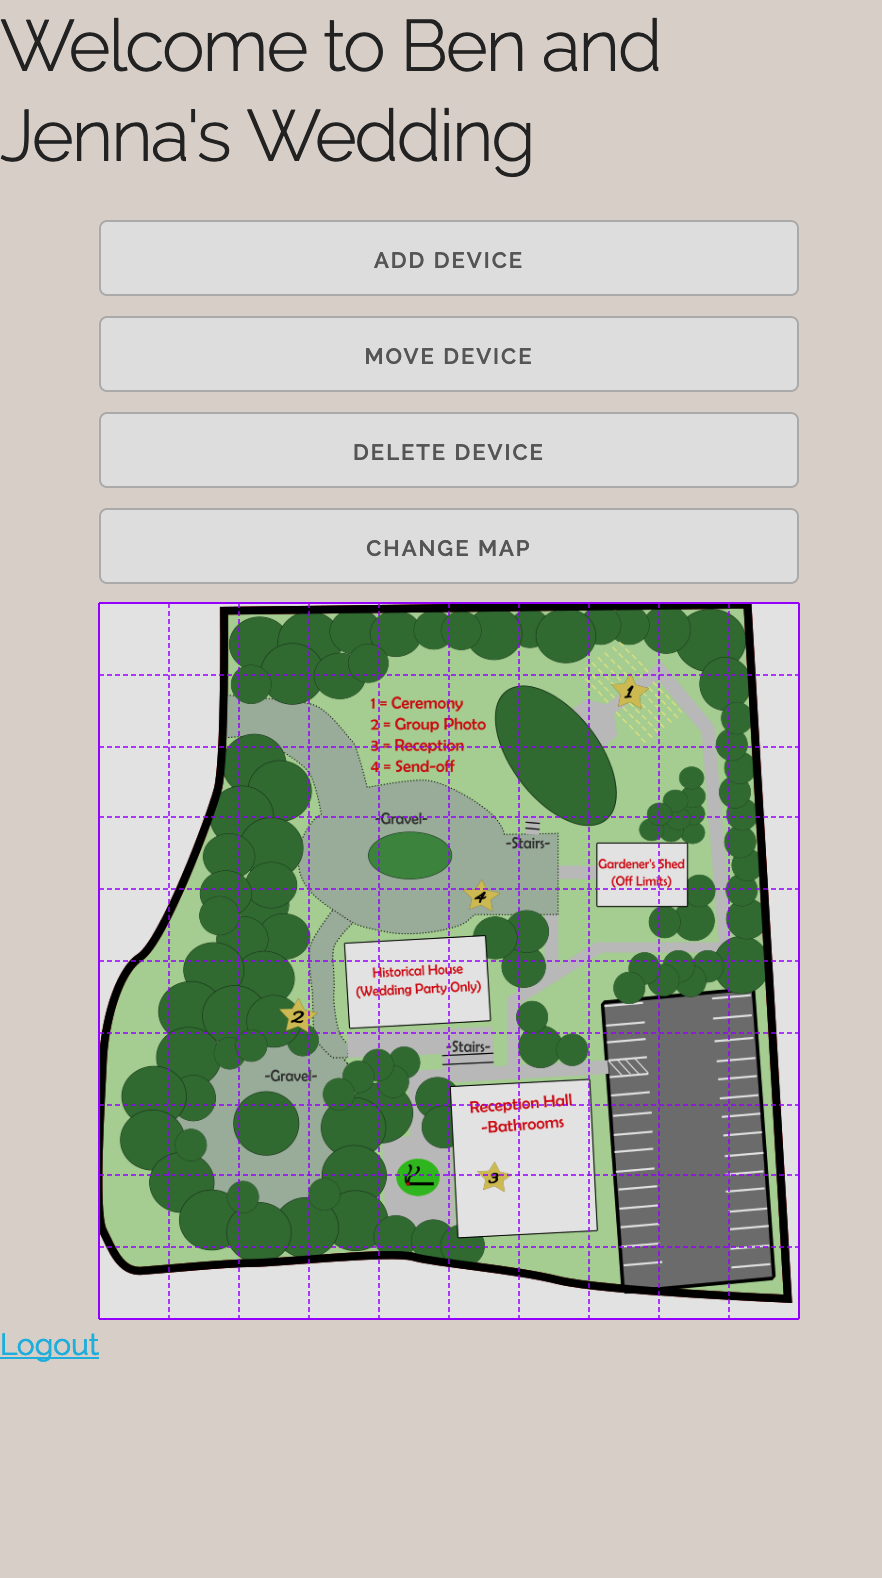
\includegraphics[scale=0.24]{Images/admin-view-mobile-grid.png}
            \centering\caption{Grid on Mobile Size}
            \label{fig:Change}
        \end{figure}
    
    \subsection{User Study}
    We conducted our first user study with a student where English is not their first language.
    During the study we had them test all of the functionalities of the webpage.
    First, the student logged into the webportal using the "viewer" token.
    There was some difficulty in conveying what we wanted them to do, but after they understood they were able to login without any hindrances.
    Then we had the student select one of the cameras to view the stream and log out of the viewer page, which they were able to do without any difficulty.
    After that we had them log in again, this time with the "admin" token.
    Once they logged into the admin page, we had them test all of the available funcitonalities including adding, moving, and deleting a device as well as updating the map.
    The student was able to complete all of these tasks without any notable difficulties.
    The user study revealed that we need to move the "back" button on the webpage to the same location as the logout button. 
    This was discovered when the student continuously used the back button on their browser ribbon to return to the previous page instead of the one on the website.
    Overall, the webpage is well formatted and is easy to operate, which is one of the teams main goals.

\begin{thebibliography}{1}

\bibitem{IEEEhowto:TravelBan}
 Liptak, A. and Shear, M. (2018). Trump’s Travel Ban Is Upheld by Supreme Court. [online] Nytimes.com. Available at: https://www.nytimes.com/2018/06/26/us/politics/supreme-court-trump-travel-ban.html?module=inline [Accessed 12 Oct. 2018].

\end{thebibliography}
\end{document}
